% begin module volumes-otherline
\begin{frame}
\begin{example}[Rotation About Line Parallel to $x$-axis]
Find the volume of the solid obtained by rotating about the line $y = 1$ \alert<handout:0| 4>{the region bounded by \alert<handout:0| 2>{$y = -x^2+2x+1$} and \alert<handout:0| 3>{$y = 1$}.}

\uncover<5->{%
Cross-section: a circle centered at $(x, 1)$, radius: $(-x^2+2x+1)-1 $, area: $\pi \left((-x^2+2x+1)-1  \right)^2 =\pi \left(-x^2+2x  \right)^2 $.
}%

\begin{columns}[c]
\column{0.35\textwidth}
\begin{pspicture}(-1,-2)(3,3)%
\tiny%
\fcBoundingBox{-1}{-0.7}{2.5}{2.5}%
\newcommand{\theFun}{u u mul -1 mul 2 u mul add 1 add\space}%
\newcommand{\theYAxis}{1\space}%
\newcommand{\theSurfaceFla}{u v cos \theFun \theYAxis sub mul \theYAxis add v sin \theFun \theYAxis sub mul\space}%
\newcommand{\theSurface}{%
\fcSurfaceInScene[colorVU= {0.7 0.2 0.2}, iterationsU=4, arrows=none, linewidth=0.3, linecolor=black ]{0.03}{0}{1.99}{30 \fcIterationsV\space mul}{[\theSurfaceFla]}{}%
}%
\renewcommand{\fcScreenStyle}{x}%
\renewcommand{\fcScreen}{[0 0 -1] 0}%
\renewcommand{\fcIterationsU}{4}%
\only<handout:2|4->{\renewcommand{\fcScreen}{[-0.03 -0.03 -1] 0}}%
\only<handout:2|5->{\renewcommand{\fcScreen}{[-0.06 -0.06 -1] 0}}%
\only<handout:2|6->{\renewcommand{\fcScreen}{[-0.12 -0.12 -1] 0}}%
\only<handout:2,3|7->{\renewcommand{\fcScreen}{[-0.15 -0.15 -1] 0}}%
\fcStartIIIdScene%
\only<handout:3|12->{%
\fcSurfaceInScene[colorUV=cyan, colorVU=cyan, linecolor=cyan, arrows=(none), iterationsV=22]{1.02 }{0 }{1 dict begin /u 0.5 def \theFun end }{ 360}{ [0.5 v cos u 1 sub  mul 1 add v sin u 1 sub mul] }{}%
}%
\only<handout:2|10,11>{%
\renewcommand{\fcIterationsV}{12}%
\theSurface%
}%
\only<handout:2,3|11,12->{\fcCurveIIIdInScene[linecolor=blue, linewidth=1]{0}{360}{2 dict begin /v t def /u 0.5 def [\theSurfaceFla] end}}%
\fcAxesIIId[zLabel={}, arrows=->]{2.2}{2.2}{3}%
\fcPutIIId[t]{[0 0 3.1]}{$z$}%
\only<handout:0|8>{%
\renewcommand{\fcIterationsV}{3}%
\theSurface%
\fcCurveIIIdInScene[arrows=(none), linecolor=red, linewidth=1.5]{0}{2}{[2 dict begin /v 90 def /u t def \theSurfaceFla end]}%
}%
\only<handout:2|9>{%
\renewcommand{\fcIterationsV}{6}%
\theSurface%
\fcCurveIIIdInScene[arrows=(none), linecolor=red, linewidth=1.5]{0}{2}{[2 dict begin /v 180 def /u t def \theSurfaceFla end]}%
}%
\only<3->{\fcCurveIIIdInScene[arrows=(none), linecolor=red, linewidth=1.5]{0}{2}{[1 dict begin /u t def t \theFun 0 end]}}%
\fcLineIIIdInScene[linecolor=red, linewidth=1, arrows= (none)]{ [0 1 0]}{[2 1 0]}%
\fcFinishIIIdScene%
\only<12->{%
\fcDotIIId{[0.5 1 0]}%
\fcPutIIId[lt]{[0.6 0.9 0]}{$(x,1)$}%
}%
\fcPutIIId[b]{[1.3 2.2 0]}{$y=-x^2+2x+1$}
\uncover<13->{\fcLineIIId[linecolor=red]{[0.5 1 0]}{[0.5 1 dict begin /u 0.5 def \theFun end  0]}}
\end{pspicture}
%\only<handout:0| 1>{%
%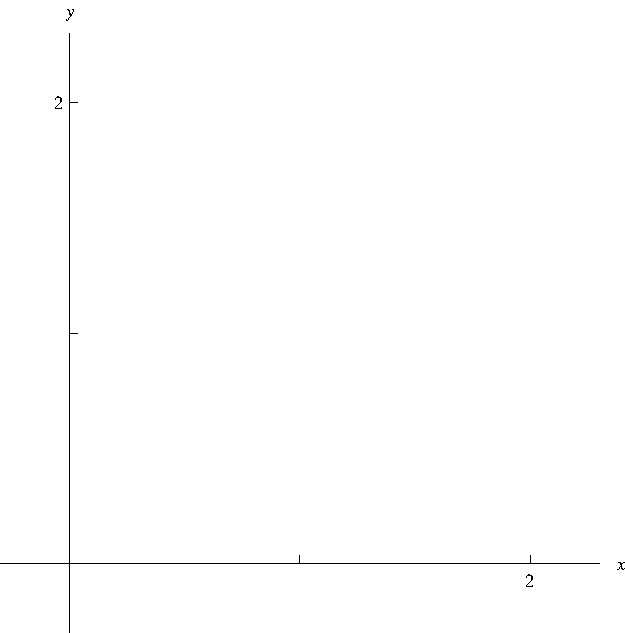
\includegraphics[height=2cm]{volumes/pictures/06-02-otherlinea.pdf} %
%}%
%\only<handout:0| 2>{%
%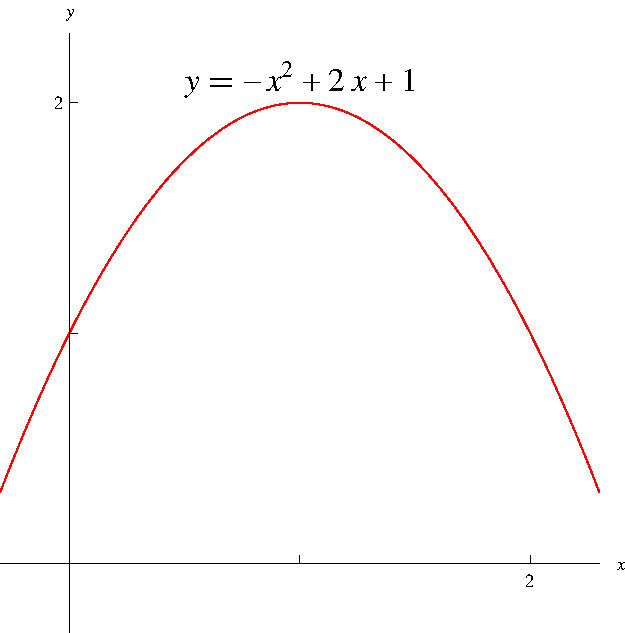
\includegraphics[height=2cm]{volumes/pictures/06-02-otherlineb.pdf} %
%}%
%\only<handout:0| 3>{%
%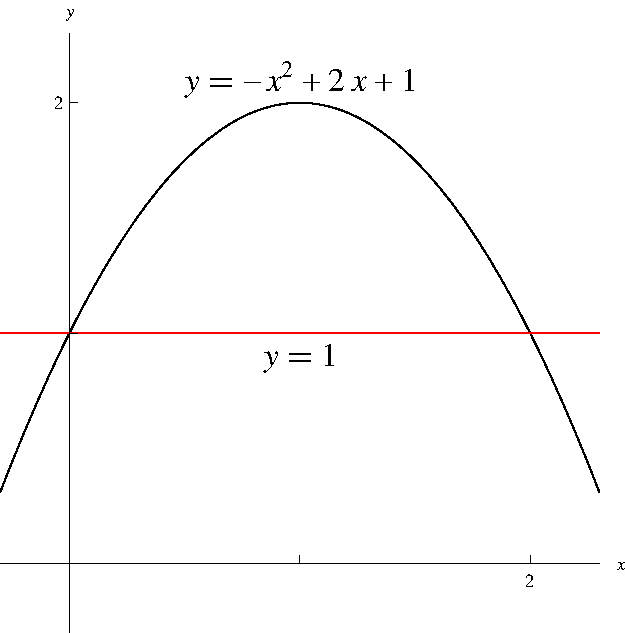
\includegraphics[height=2cm]{volumes/pictures/06-02-otherlinec.pdf} %
%}%
%\only<handout:0| 4>{%
%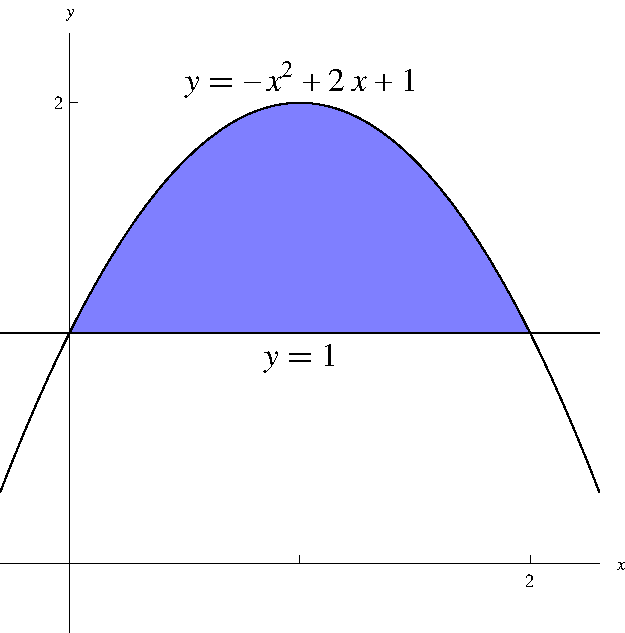
\includegraphics[height=2cm]{volumes/pictures/06-02-otherlined.pdf} %
%}%
%\only<5->{%
%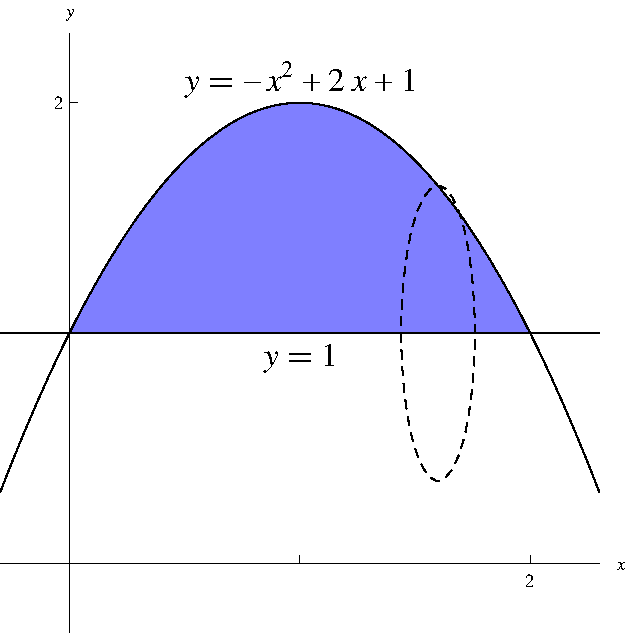
\includegraphics[height=2cm]{volumes/pictures/06-02-otherlinee.pdf} %
%}%
\column{0.65\textwidth}

\uncover<handout:3|1->{
$
\begin{array}{@{}r@{~}c@{~}l}
\uncover<8->{V&  = &\displaystyle \int_{0}^{2}A(x)\diff x= \int_0^2  \pi \left( -x^2+2x\right)^2  \ \diff x%
}\\%
\uncover<9->{&  = &\displaystyle \pi \int_0^2 \left( \alert<handout:0| 10-11>{x^4} - \alertNoH{12-13}{4x^3} + \alertNoH{14-15}{4x^2} \right)  \diff x }\\%
\uncover<10->{&  =& \displaystyle \pi {\left[ \fcAnswerUncover{10}{11}{ \frac{ x^5 }{5}} - \fcAnswerUncover{10}{13}{x^4} + \fcAnswerUncover{10}{15}{ \frac{4 x^3}{3}} \right]}_0^2%
}\\%
\uncover<16->{&  = &\displaystyle  \pi \left( \frac{32}{5} - 16 + \frac{32}{3} \right) \uncover<17->{= \frac{16}{15}\pi}
}%
\end{array}
$
}
\end{columns}
\end{example}
\end{frame}
% end module volumes-otherline
